\documentclass[tikz]{standalone}
\usepackage{tikz}
\usetikzlibrary{automata,positioning,arrows.meta}
\tikzset{
    >=Stealth,
    every edge/.style={draw,->,>=Stealth,thick},
    every loop/.style={draw,->,>=Stealth,thick}
}
\begin{document}

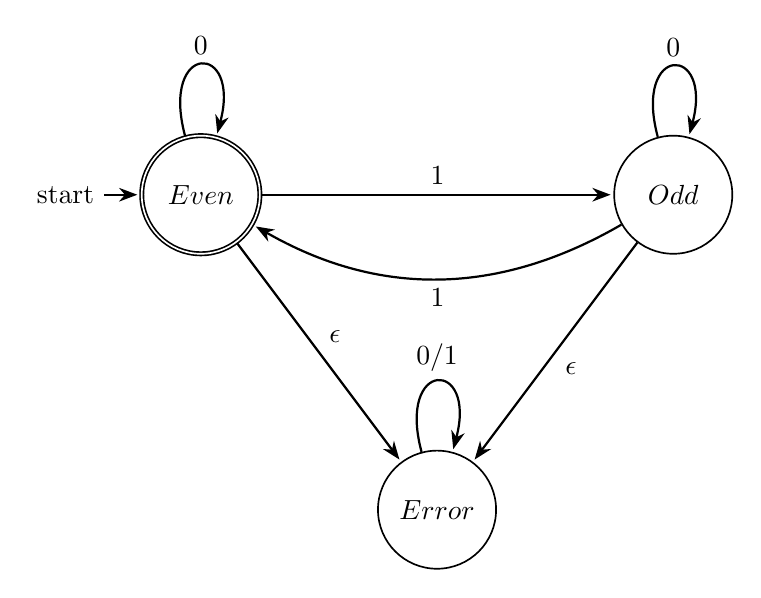
\begin{tikzpicture}[shorten >=1pt,auto,node distance=3cm,
                    semithick,
                    state/.style={circle,draw,minimum size=1.5cm}]

% States
\node[state,initial,accepting] (q1) at (0.00cm,0.00cm) {$Even$};
\node[state] (q2) at (6.00cm,0.00cm) {$Odd$};
\node[state] (q3) at (3.00cm,-4.00cm) {$Error$};

% Transitions
\path (q1) edge [loop above] node {$0$} (q1);
\path (q1) edge node {$1$} (q2);
\path (q2) edge [loop above] node {$0$} (q2);
\path (q2) edge [bend left=30] node {$1$} (q1);
\path (q1) edge node {$\epsilon$} (q3);
\path (q2) edge node {$\epsilon$} (q3);
\path (q3) edge [loop above] node {$0/1$} (q3);

\end{tikzpicture}
\end{document}
